\documentclass[11pt,a4paper]{article}
\usepackage[margin=0.8in,top=1in]{geometry}
\usepackage{amsmath,amssymb}
\usepackage{graphicx}

\newcommand{\bE}{\mathbb{E}}

\pagestyle{empty}

\begin{document}
\noindent\fbox{%
  \begin{minipage}{\dimexpr\textwidth-2\fboxsep-2\fboxrule\relax}
    \vspace{6pt}
    \hspace{6pt}\textbf{Machine Learning 1}
    \begin{center}
      \Large Homework 1
    \end{center}
    \vspace{6pt}
  \end{minipage}%
}

\section{problem 1}
\paragraph{1(a).} Since $\bE_{X\sim P}[U(a,X)]=(d+\frac{2}{3}a)*0.85+(d-a)*0.15=d+\frac{5}{12}a$ and $0\leq a\leq d$, we have $a^\ast =d$. If it takes variance/risk of bet into account it would make more sense.
\paragraph{1(b).} Since $\bE_{X\sim P}[U(a,X)]=\log(d+\frac{2}{3}a)*0.85+\log(d-a)*0.15$, 
\[
f(a)=\log(d+\frac{2}{3}a)*0.85+\log(d-a)*0.15, f'(a)=\frac{17}{30}/(\frac{2}{3}a+d)-0.15/(d-a)
\]
solve $f'(a)=0$ we have $a^*=0.625d$, and furtheremore $f''(a^*)<0$. 
\paragraph{1(c).} No. I am personally more risk-averse.
\section{problem 2}
Note that 
\begin{align*}
  \arg\min\bE_{X,Y}[L(Y,f(X))]&=\arg\min\bE_{X,Y}[-Y\log f(X)-(1-Y)\log (1-f(X))]\\
  &=\arg\min \bE_{X}[\bE_{Y|X}[-Y\log f(X)-(1-Y)\log (1-f(X))|X]]\\
  &=\arg\min \bE_{X}[-p(Y=1|X)\log f(X)-(1-p(Y=1|X=x))\log (1-f(X))]
\end{align*}
take derivative with respect to $f(x)$ gives $f^\ast(x)=p(Y=1|X=x)$ and furthermore the second derivative is negative, which concludes the result.

\section{problem 3}
One of the reason that there is already bias comes from the finite sample compared to ground truth distribution, so in such case we only need to achieve a loss with same order as sampling bias instead of a zero loss.

\clearpage
\section{problem 4}
Lets just focus on the fitted residual on train/test data. We use 5 different models including linear regrassion, support vector regrassion, decision tree, random forest and neural network. We present qq plot and a normal test of five models.
\paragraph{Test residuals ($n=22$).}
\begin{center}
  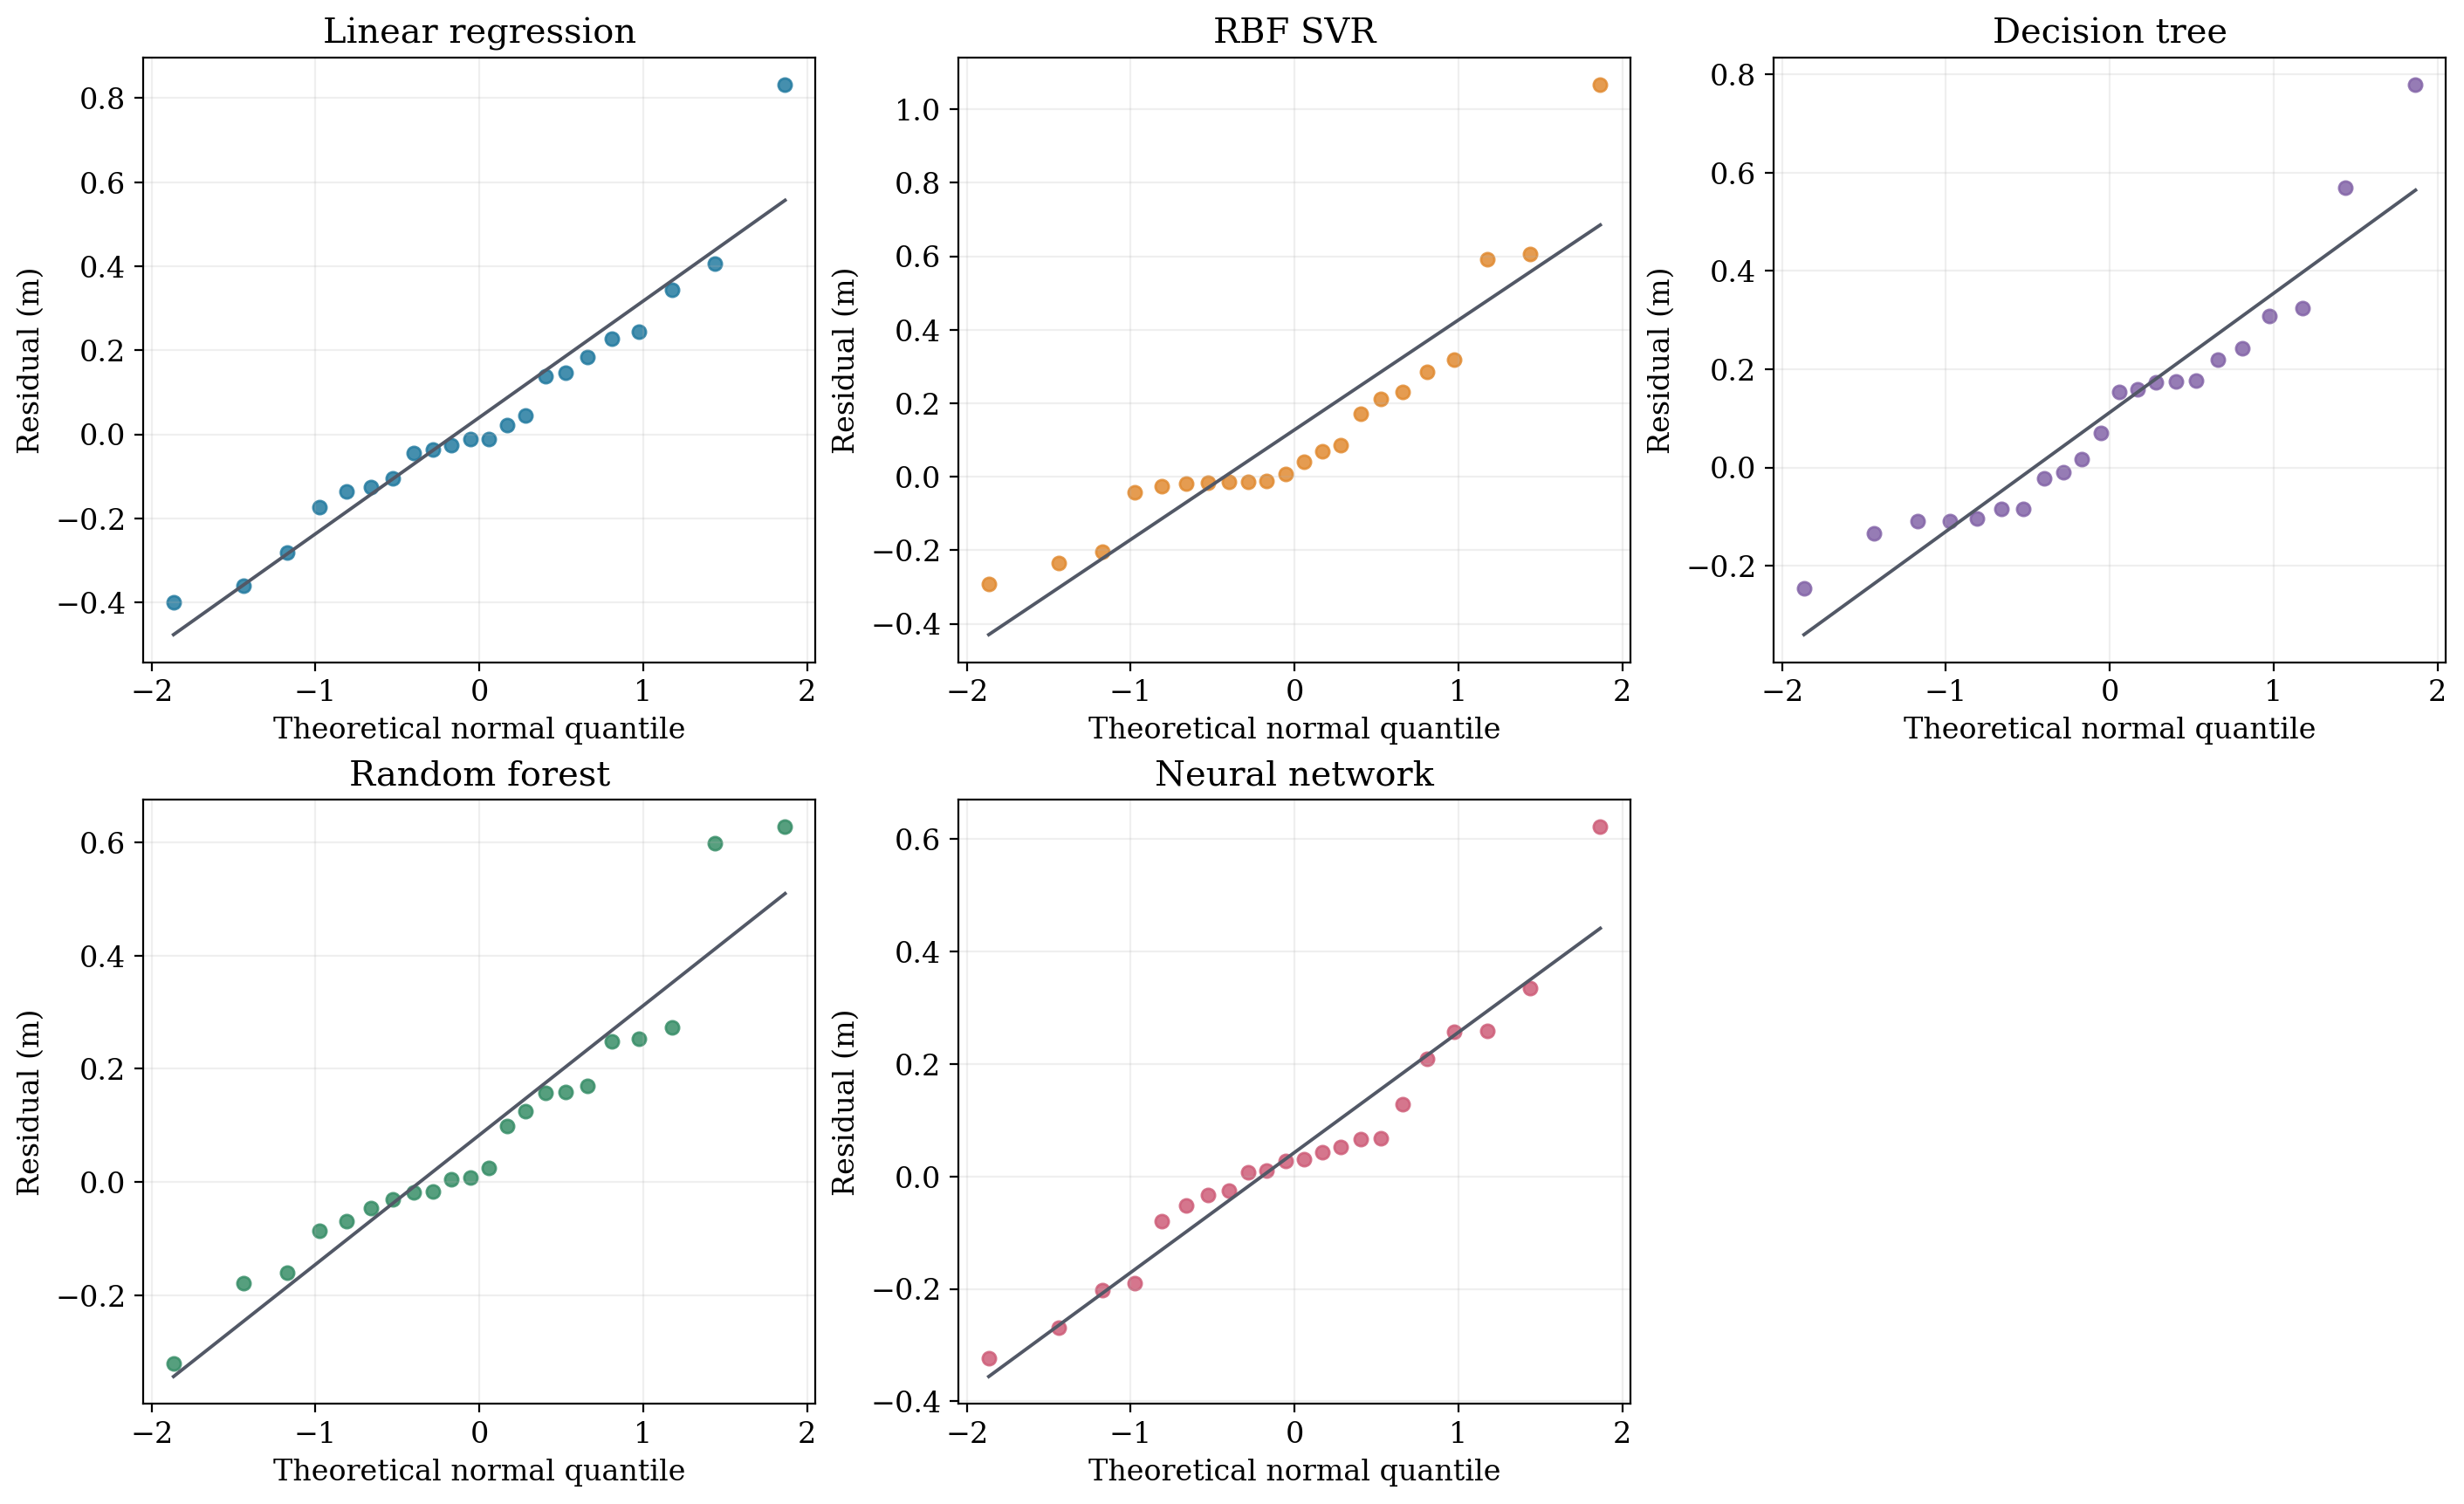
\includegraphics[width=\textwidth]{problem4_ale/figures/qq_test_hw1.png}

  \vspace{8pt}
  \begin{tabular}{lrr}
    \hline
    Model & \texttt{normaltest} $K^2$ & $p$-value \\
    \hline
    Linear regression & 7.2997 & 0.025995 \\
    RBF SVR           & 13.0913 & 0.001436 \\
    Decision tree     & 7.0637 & 0.029250 \\
    Random forest     & 5.1604 & 0.075758 \\
    Neural network    & 4.8691 & 0.087637 \\
    \hline
  \end{tabular}
\end{center}

\clearpage
\paragraph{Training residuals ($n=85$).}
\begin{center}
  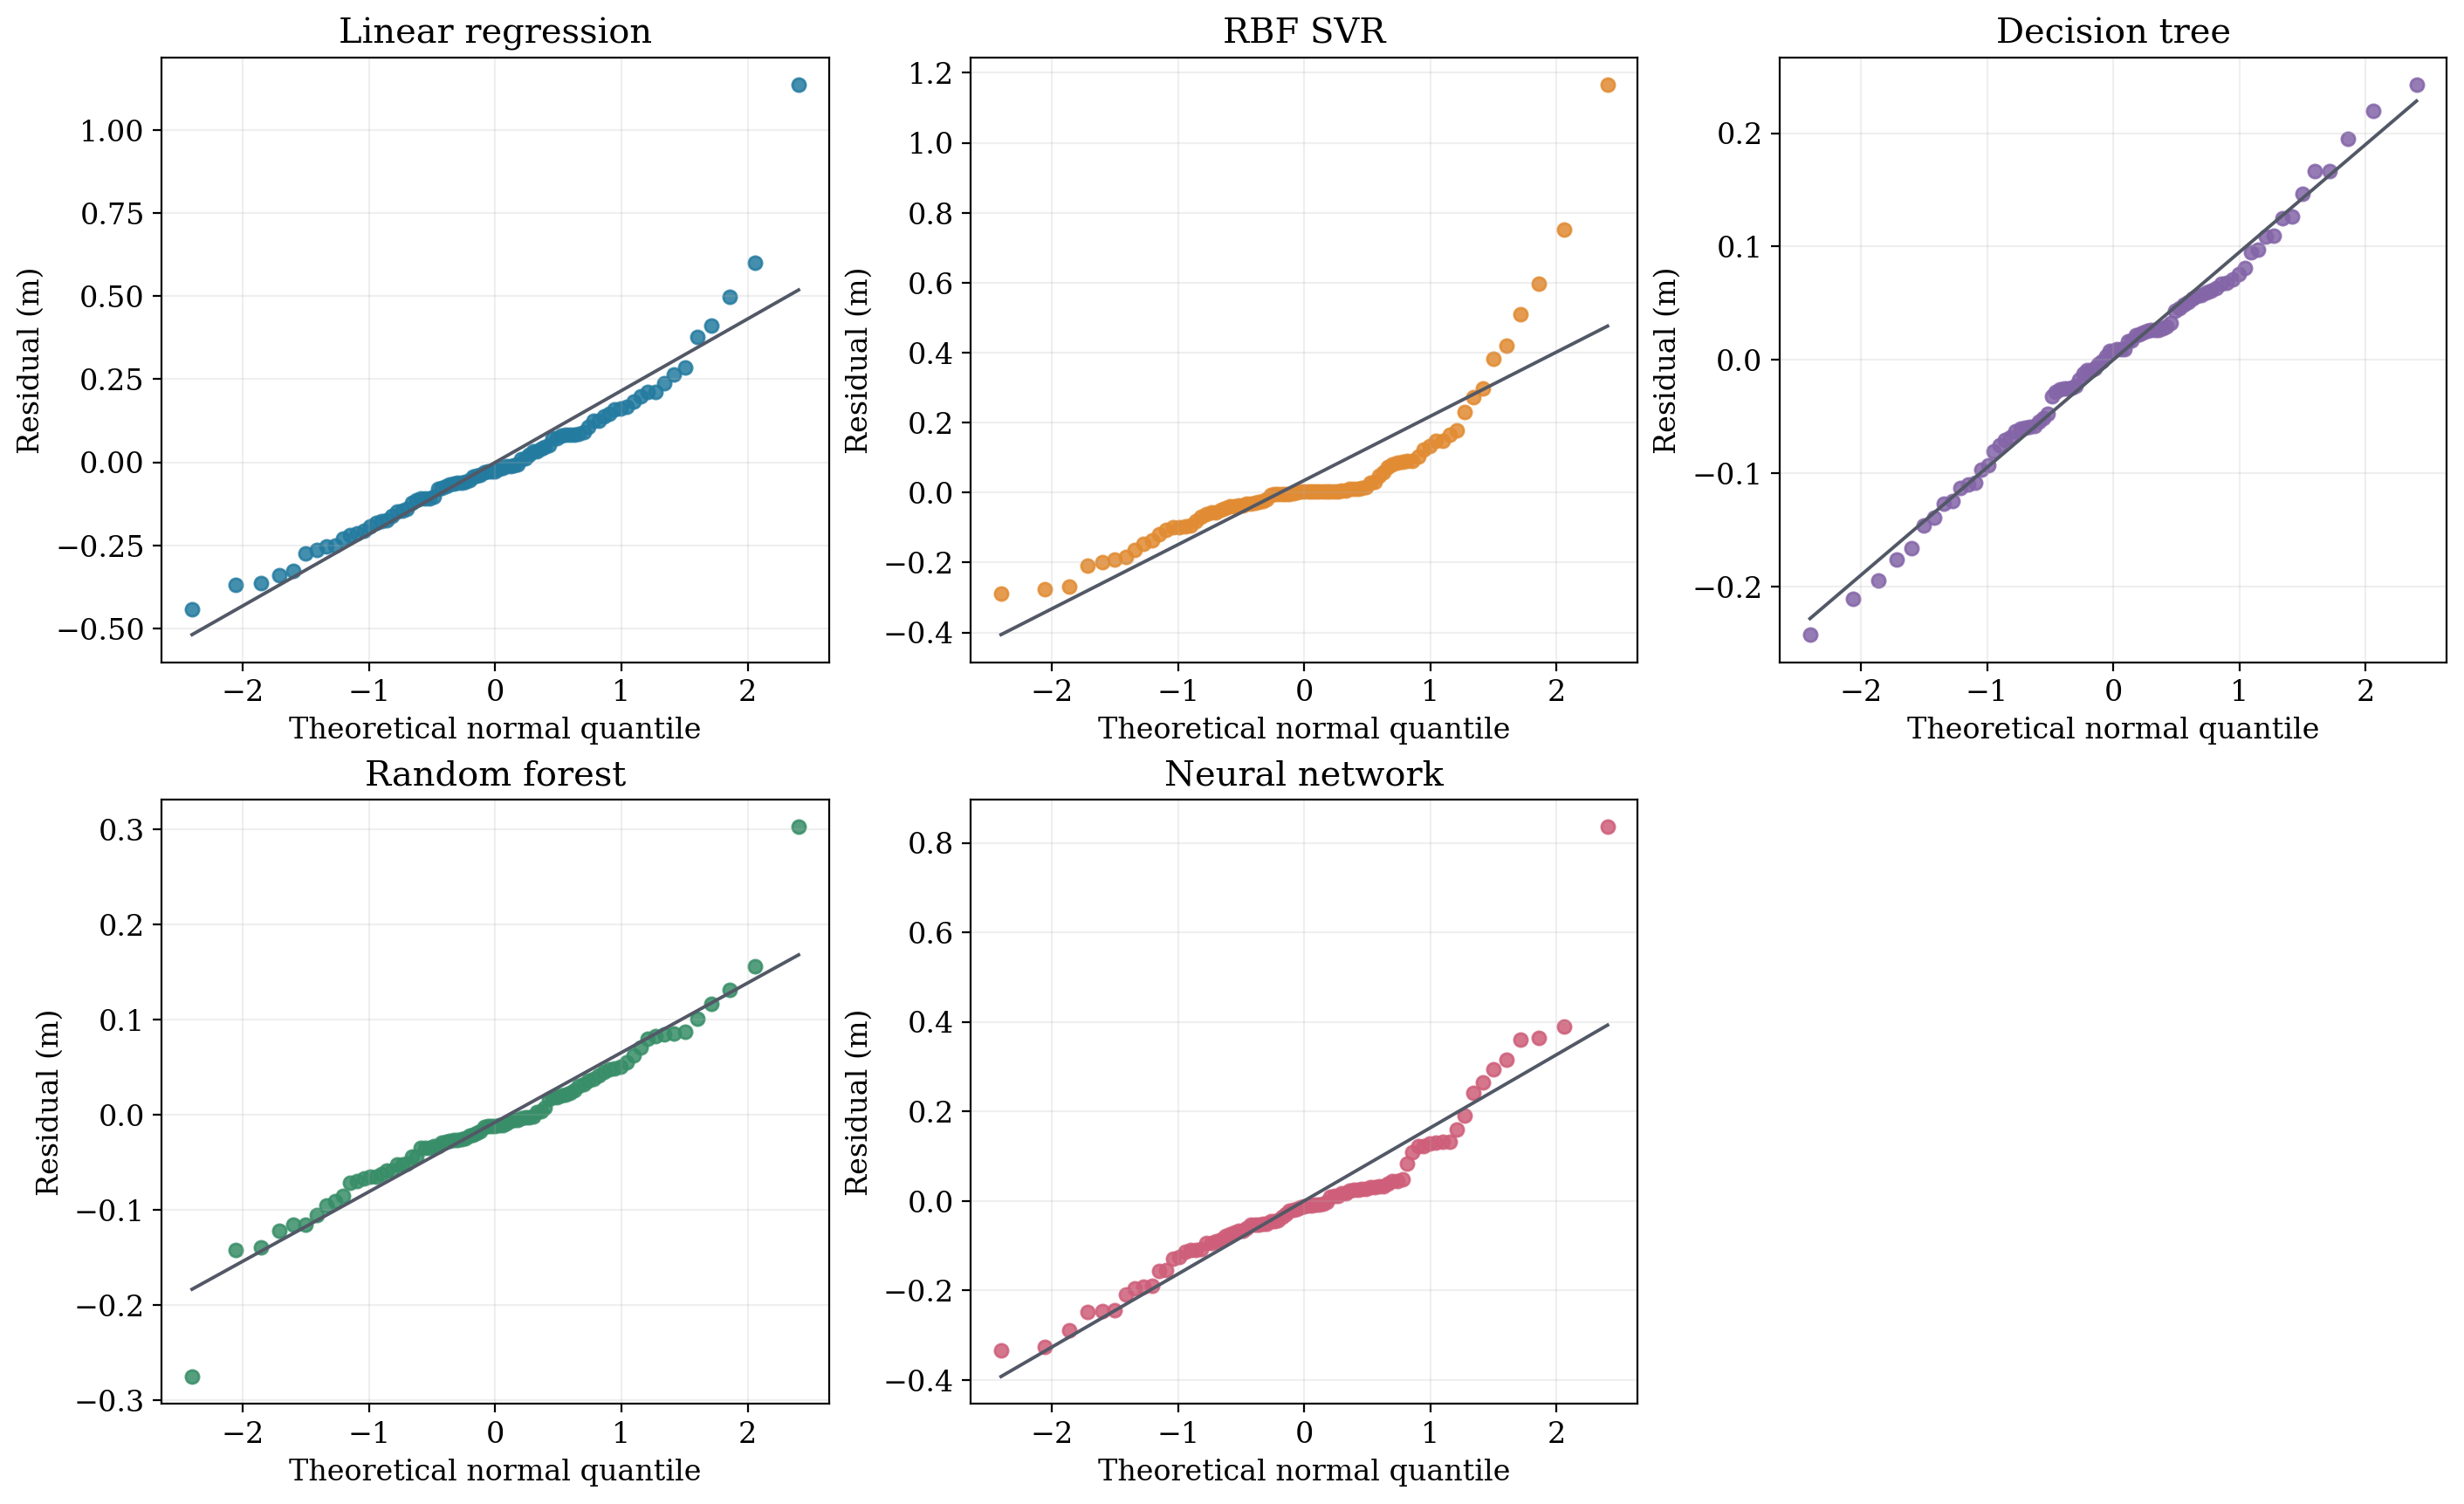
\includegraphics[width=\textwidth]{problem4_ale/figures/qq_train_hw1.png}

  \vspace{8pt}
  \begin{tabular}{lrr}
    \hline
    Model & \texttt{normaltest} $K^2$ & $p$-value \\
    \hline
    Linear regression & 46.5802 & $7.678\times10^{-11}$ \\
    RBF SVR           & 71.4519 & $3.051\times10^{-16}$ \\
    Decision tree     & 0.8014 & 0.669853 \\
    Random forest     & 16.2658 & $2.937\times10^{-4}$ \\
    Neural network    & 42.2184 & $6.798\times10^{-10}$ \\
    \hline
  \end{tabular}
\end{center}
On test set, for linear regression, SVR and dicision tree, we reject the hepothesis of a normal residual under significance level $0.05$. The qq plot also exhibits a deviation on the tail. On train set, we reject all the model except decision tree. However the decision tree has a strong overfitting on train set.
\clearpage
\section{problem 5}
Both datasets use an 80/20 split with seed 42. We compare 200 and 500 epochs along the same SGD trajectory with mini-batch shuffle seed 42. Each model uses its full training set with fixed hyperparameters, without cross-validation. Features are standardized using training data only. Classification probabilities are clipped to $[10^{-6},1-10^{-6}]$ before BCE; gradient norms are clipped at 5. The learning rate is $\eta_e=\eta_0/(1+e/100)$, where $e$ starts at zero.

\paragraph{Classification ($n_{\mathrm{train}}=455$, $n_{\mathrm{test}}=114$).}
\begin{center}
  \begin{tabular}{lrrrr}
    \hline
    Model & Epochs & Correct & Test accuracy & $\Delta$ accuracy \\
    \hline
    sklearn logistic (L2) & $-$ & 112/114 & 0.9825 & +0.0000 \\
    PyTorch logistic (SGD) & 200 & 110/114 & 0.9649 & -0.0175 \\
    PyTorch logistic (SGD) & 500 & 110/114 & 0.9649 & -0.0175 \\
    PyTorch probit (SGD) & 200 & 109/114 & 0.9561 & -0.0263 \\
    PyTorch probit (SGD) & 500 & 110/114 & 0.9649 & -0.0175 \\
    \hline
  \end{tabular}
\end{center}

For the additional test metrics, malignant ($y=0$) is the positive class. ROC-AUC uses its predicted probability; $F_1$, sensitivity, and specificity use the same 0.5 classification threshold. Higher values are better.

\begin{center}
  \begin{tabular}{lrrrrr}
    \hline
    Model & Epochs & ROC-AUC & $F_1$ & Sensitivity & Specificity \\
    \hline
    sklearn logistic (L2) & $-$ & 0.9954 & 0.9762 & 0.9762 & 0.9861 \\
    PyTorch logistic (SGD) & 200 & 0.9954 & 0.9535 & 0.9762 & 0.9583 \\
    PyTorch logistic (SGD) & 500 & 0.9957 & 0.9535 & 0.9762 & 0.9583 \\
    PyTorch probit (SGD) & 200 & 0.9954 & 0.9425 & 0.9762 & 0.9444 \\
    PyTorch probit (SGD) & 500 & 0.9954 & 0.9535 & 0.9762 & 0.9583 \\
    \hline
  \end{tabular}
\end{center}

\paragraph{Classification (a).} SGD uses batch size 64, initial learning rate 0.05, and momentum 0. The sigmoid model achieves 96.49\% accuracy at both 200 and 500 epochs, 1.75 percentage points below the baseline. ROC-AUC is almost identical to the baseline. Sensitivity is also identical, while specificity is lower: the model produces three false positives, compared with one for sklearn. The PyTorch model minimizes BCE without a penalty; sklearn uses L2 regularization.

\paragraph{Classification (b).} With the same SGD settings, replacing sigmoid with the standard normal CDF improves accuracy from 95.61\% at 200 epochs to 96.49\% at 500 epochs. False positives decrease from four to three; sensitivity is unchanged. The 500-epoch result remains 1.75 percentage points below the baseline, with almost identical ROC-AUC. Both models use clipped BCE.

\clearpage
\paragraph{Regression ($n_{\mathrm{train}}=85$, $n_{\mathrm{test}}=22$).}
\begin{center}
  \begin{tabular}{lrrr}
    \hline
    Model & Epochs & Test MAE (m) & $\Delta$ MAE (m) \\
    \hline
    sklearn linear & $-$ & 0.195393 & +0.000000 \\
    PyTorch linear (MSE, SGD) & 200 & 0.195232 & -0.000161 \\
    PyTorch linear (MSE, SGD) & 500 & 0.195753 & +0.000360 \\
    PyTorch linear ($t_5$ NLL, SGD) & 200 & 0.194035 & -0.001358 \\
    PyTorch linear ($t_5$ NLL, SGD) & 500 & 0.194308 & -0.001086 \\
    \hline
  \end{tabular}
\end{center}

RMSE gives greater weight to large errors than MAE; lower is better. Higher $R^2$ indicates better fit relative to a constant predictor using the test-set mean.

\begin{center}
  \begin{tabular}{lrrr}
    \hline
    Model & Epochs & Test RMSE (m) & Test $R^2$ \\
    \hline
    sklearn linear & $-$ & 0.270543 & 0.629198 \\
    PyTorch linear (MSE, SGD) & 200 & 0.270485 & 0.629356 \\
    PyTorch linear (MSE, SGD) & 500 & 0.269541 & 0.631939 \\
    PyTorch linear ($t_5$ NLL, SGD) & 200 & 0.272995 & 0.622445 \\
    PyTorch linear ($t_5$ NLL, SGD) & 500 & 0.272095 & 0.624931 \\
    \hline
  \end{tabular}
\end{center}

\paragraph{Regression (a).} SGD uses batch size 32, initial learning rate 0.03, and momentum 0. With MSE, test MAE is 0.195232 m at 200 epochs and 0.195753 m at 500 epochs, compared with 0.195393 m for the baseline. The 500-epoch model has slightly lower RMSE and higher $R^2$ than the baseline, despite its slightly higher MAE. These small differences are consistent with finite stochastic updates near the least-squares solution.

\paragraph{Regression (b).} With the same SGD settings, minimizing the Student-$t$ negative log-likelihood with $\nu=5$ and fixed scale 1 gives test MAE 0.194035 m at 200 epochs and 0.194308 m at 500 epochs. Both are lower than the baseline, but their RMSE is higher and $R^2$ is lower. Thus, the improvement depends on the evaluation metric. ALE remains in its original units.
\end{document}
